\documentclass{article}

\usepackage{silence}
\WarningFilter{latex}{You have requested package}

\usepackage[T1]{fontenc}
\usepackage[unicode,hidelinks]{hyperref}
\usepackage{tikz}
\usepackage{tikzuml/tikz-uml}
\usepackage{graphicx}
\usepackage{fancyhdr}
\pagestyle{fancy}

\usetikzlibrary{positioning}
\usetikzlibrary{fit}
\usetikzlibrary{scopes}
\usetikzlibrary{calc}

\newcommand{\projectname}{Graphkasten}

\tikzset{note/.style={circle,draw=black,fill=orange,thick,minimum size=2em},
	selected/.style={circle,thick,draw=blue,minimum size=2.7em},
	link/.style={draw=black},
	arrow/.style={->,draw=blue,thick},
	arrow_letter/.style={blue},
	outline/.style={draw=red,thick}}

\title{\projectname}
\author{Kryštof Albrecht \\ \href{mailto:krystofalbrechtus@gmail.com}{krystofalbrechtus@gmail.com}}

\begin{document}
\maketitle
\tableofcontents

\newpage

\section{Introduction}

\projectname\ provides a \emph{graph view} of the notes, \emph{keyboard-driven navigation} and \emph{flexible search} to refine interaction with a Vimwiki-based Zettelkasten.

\subsection{Motivation}

Tools like Vimwiki, Vimzettel and Taskwiki provide a solid base for a Zettelkasten workflow. These are based on \emph{the Vim text editor}, which has a lot of advantages:

\begin{itemize}
	\item Text editing cannot be faster
	
	\item Adding new notes is effortless

	\item The system is simple

	\item Tasks can have note links in them

	\item Any missing functionality can be added through Vimscript
\end{itemize}

The problem is however, that there is no GUI. Tools like \emph{Obsidian} offer a \emph{graph view} that enables natural viewing of the \emph{networked structure} of the Zettelkasten. This view allows faster and easier search and navigation, but also improves the chances of \emph{emergent ideas.}


\begin{center}
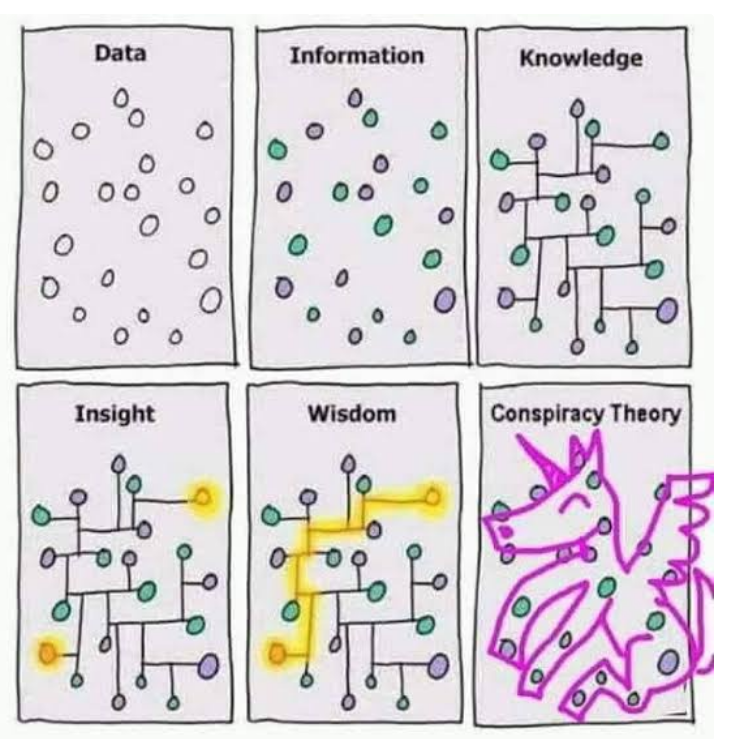
\includegraphics[width=\linewidth/2]{fig/wisdom.png}
\end{center}

\newpage

\subsection{Use case diagram}\label{sec:use_case_diagram}

The note\footnote{The terms \emph{node} and \emph{note} are used interchangeably throughout this document.} graph is \emph{the basis} of the system and \emph{all} of the use cases are related to it. 

\begin{center}
\begin{tikzpicture}
	\umlactor[y=-2]{User}

	\begin{umlsystem}[x=4]{\projectname}
		\umlusecase[y=1]{Search notes (\ref{gelement:notes})}
		\umlusecase[x=4]{Show result in graph (\ref{gelement:lenses})}

		\umlusecase[y=-1]{Highlight close nodes}

		\umlusecase[y=-3]{Show HTML preview}
		\umlusecase[y=-4,x=4]{Highlight hovered link}

		\umlusecase[y=-2]{Open note in Neovim}
		\umlusecase[y=-5,x=1]{Select nodes within outline (\ref{gelement:outlines})}
		\umlusecase[y=-6,x=1,fill=white]{Open calendar/timeline (v2)}
	\end{umlsystem}

	\umlextend{usecase-2}{usecase-1}
	\umlinclude{usecase-4}{usecase-5}

	\umlassoc{User}{usecase-1}
	\umlassoc{User}{usecase-3}
	\umlassoc{User}{usecase-4}
	\umlassoc{User}{usecase-6}
	\umlassoc{User}{usecase-7}
	\umlassoc{User}{usecase-8}
\end{tikzpicture}
\end{center}

\subsection{Miscellaneous features}

Apart from the aforementioned main use cases, there will also be the following features:

\begin{itemize}
	\item Showing files/attachments in the graph view

	\item Support for Vimwiki tags

	\item Real-time updates

	\item Fast search
\end{itemize}

\newpage

\subsection{Common scenarios} % TODO Add pictures to scenarios

Here are a few scenarios of how using the application might play out.

\subsubsection{Processing the staging area}

I've taken some notes and put them into the Staging Area. Now I want to quickly integrate them into the Zettelkasten.

\begin{enumerate}
	\item The staged notes have an \emph{outline} around them in the graph view. Each staging subtask is \emph{further divided} by outlines.

	\item I \emph{highlight} all the task notes within an outline.

	\item I \emph{open} all the notes at once in Neovim with a single click.

	\item I can view the HTML preview of the note I am working on.

	\item As I work, the graph updates \emph{in real time}.
\end{enumerate}

\subsubsection{Searching for information}

I need to query some information in the Zettelkasten.

\begin{enumerate}
	\item I enter my search query by \emph{just starting to type.}

	\item The graph updates in real time and shows just the nodes matching the query. 

	\item I have the option to show a small snippet of the note next to each node.

	\item The most relevant node is highlighted and its HTML preview is shown automatically.

	\item Hitting ENTER, I can navigate the nodes with \emph{Vim keys}.

	\item Hitting ENTER again, I can navigate the HTML preview.
\end{enumerate}

\newpage

\section{Architecture}

\subsection{UI Overview}\label{sec:ui_layout}

The note graph is \emph{the basis} of the system and so will always be shown. The user will then be able to \emph{adjust} this graph view. Any other view will open as a sidebar.

\newcommand{\drawborder}{
	\node[fit={(0,0) (\linewidth, 0.5625\linewidth)}, draw=black, thick, outer sep=0](border){};
}

\newcommand{\uicontainer}[3]{
	\node[fit={#1 #2}, inner sep=0, outer sep=0](#3){};
}

\newcommand{\uielement}[5]{
	\uicontainer{#1}{#2}{#4}

	\node[fit={(#4.north west) (#4.south east)}, draw=#3, fill=#3, fill opacity=0.05, thick, inner sep=-0.3]{};
	\node[text=#3] at (#4){#5};
}

\begin{center}

\begin{tikzpicture}[scale=0.95]
	% Draw screen border (optimized for 1920x1080)
	\drawborder

	% Draw the UI elements
	%% HTML Preview
	\uielement{($(border.south east) - (10em, 0)$)}{(border.north east)}{red}{preview}{\hyperref[sec:html_preview]{HTML Preview}}

	%% Graph View
	\uielement{(border.north west)}{(preview.south west)}{blue}{graph}{\hyperref[sec:graph_view]{Graph View}}

	%% Searchbar
	\uielement{($(graph.north west) + (4em, 0)$)}{($(graph.north east) - (4em, 1.2em)$)}{orange}{searchbar}{\hyperref[sec:search]{Searchbar}}

	%% Hamburger menu (attached to the searchbar)
	\path let \p1=( $(searchbar.south east) - (searchbar.north east)$ ) in coordinate (ham_end) at (-\y1, \y1);
	\uielement{(searchbar.north east)}{($(searchbar.north east) + (ham_end)$)}{magenta}{hamburger}{\hyperref[sec:options]{H}}

\end{tikzpicture}

\end{center}

The \textcolor{blue}{\emph{graph view}} is the most important part of the UI. It visualizes stored ideas and the connections between them and allows navigating related ideas easily.

The \textcolor{red}{\emph{HTML preview}} shows the currently selected note in HTML format. Search results are also highlighted on the page. Clicking links to other nodes on the page selects that node in the graph.

The \textcolor{orange}{\emph{searchbar}} allows filtering what is shown in the graph view. Nodes matching the search will be shown and the view will zoom in to fit the results. Other nodes will be hidden.

The \textcolor{magenta}{\emph{hamburger menu}} (attached to the searchbar) shows configuration options.

\newpage

\subsection{System states}

This section describes the states the system can get into through user interaction. The application can be controlled using the mouse, but also allows for full keyboard control.

\begin{center}
\begin{tikzpicture}
	\umlstateinitial[name=initial]
	\umlbasicstate[name=searching, below=2cm of initial, do=accept search query, exit=select most relevant node]{Searching}
	\umlbasicstate[name=navigating, below=4cm of searching, entry=highlight selected node, do=select relative nodes using Vim keys, exit=unhighlight selected node]{Navigating graph}
	\umlbasicstate[name=previewing, below=4cm of navigating, entry=focus preview panel, do=scroll preview using Vim keys, exit=unfocus preview panel]{Viewing HTML Preview}

	\umltrans{initial}{searching}
	\umltrans[arg=search query confirmed (ENTER)]{searching}{navigating}
	\umltrans[arg=ENTER pressed/selected node clicked]{navigating}{previewing}

	\umlHVHtrans[arm1=-4cm,arg=ESC pressed,pos=2]{previewing}{navigating}
	\umlHVHtrans[arm1=5cm,arg=ESC pressed,pos=2.5]{navigating}{searching}

\end{tikzpicture}
\end{center}


\newpage

\subsection{Graph View}\label{sec:graph_view}

This section provides an overview of the various \emph{elements} of the graph view. 

\begin{center}


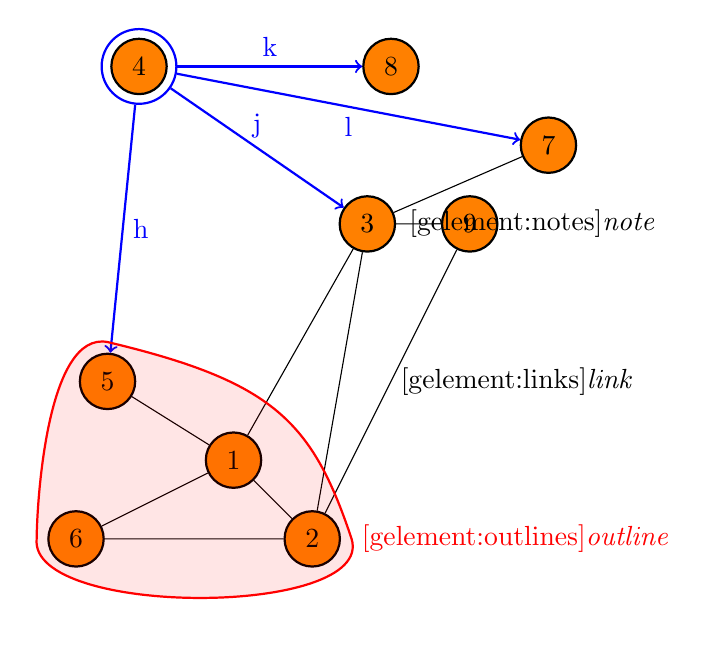
\begin{tikzpicture}
	% Draw the graph nodes
	\draw node at (0,0) [note](node1){1} 
		node at (1,-1) [note](node2){2}
		node at (1.7,3) [note](node3){3}
		node at (-1.2,5) [note](node4){4}
		node at (-1.6,1) [note](node5){5}
		node at (-2,-1) [note](node6){6}
		node at (4,4) [note](node7){7}
		node at (2,5) [note](node8){8}
		node at (3,3) [note](node9){9};

	% Draw the links between the graph nodes
	\draw[link] (node1) --(node2)
	            (node1) --(node3)
	            (node1) --(node5)
	            (node1) --(node6)
	            (node2) --(node3)
	            (node2) --(node6)
			(node2) -- node[right]{\hyperref[gelement:links]{\emph{link}}}(node9)
			(node3) --(node7)
			(node3) --(node9);
	
		% Draw a circle around the selected node
		\draw node at (node4) [selected](selected_node){};

		% Draw arrows to nodes selectable by pressing the shown key
		\draw[arrow] (selected_node) -- node[above,arrow_letter] {j} (node3);
		\draw[arrow] (selected_node) -- node[right,arrow_letter] {h} (node5);
		\draw[arrow] (selected_node) -- node[below,arrow_letter] {l} (node7);
		\draw[arrow] (selected_node) -- node[above,arrow_letter] {k} (node8);

		\draw node at ($(node9) + (0.8,0)$){\hyperref[gelement:notes]{\emph{note}}};

	% Draw outline
		\draw[outline,fill=red,fill opacity=0.1] ($(node5) + (0,0.5)$) .. controls($(node1) + (0.5,1)$) and ($(node1) + (1,0.5)$) .. ($(node2) + (0.5,0)$)

			node[right,red,fill opacity=1]{\hyperref[gelement:outlines]{\emph{outline}}}

			.. controls($(node2) + (0.8,-1)$) and ($(node6) + (-0.6,-1)$) .. ($(node6) - (0.5,0)$)

			.. controls($(node6) + (135:0.7)$) and ($(node5) + (140:1)$) .. ($(node5) + (0,0.5)$);
\end{tikzpicture}
\end{center}

\subsubsection{Notes}\label{gelement:notes}

\subsubsection{Links}\label{gelement:links}

\subsubsection{Outlines}\label{gelement:outlines}

\subsubsection{Lenses}\label{gelement:lenses}

\newpage

\subsection{Search}\label{sec:search}

\newpage

\subsection{HTML Preview}\label{sec:html_preview}

\newpage

\subsection{Options}\label{sec:options}

\newpage

\end{document}
